\documentclass[11pt,a4paper]{article}
\input{../../../../header.tex}
\input{../../../../normal.tex}

\usepackage{lmodern}
\renewcommand*\familydefault{\sfdefault} %% Only if the base font of the document is to be sans serif
\usepackage[T1]{fontenc}

\author{Kenton Lam}
\date{{MATH3202 Assignment 2 \\ Due 03/05/2019 1:00 pm}}
\title{WonderMarket \\ 
Section B -- Client Report}


\begin{document}
\maketitle
\begin{abstract}
    In this report, we propose a solution to optimise your supply chain logistics, 
    to minimise costs while ensuring all demands are met.
\end{abstract}

\part{Solution}
We have considered your requirements of weekly demand, DC capacity, surge demands, 
proposed new DCs and labour costs.
We propose the following strategy for each communication.

\section{Communication 5}
For this communication, we consider surge scenarios but without the northside capacity 
limit. 
Additionally, we require each store to be assigned to only one distribution centre. 

This resulted in a cost of \$205688 per week with the assignments below. This is \$6901 
more expensive than communication 4, which means the requirement of one DC per store 
costs more than the savings from removing the northside limit.\\[1em]
\begin{tabular}{l  r  r  r }
    Store & DC0 & DC1 & DC2 \\
    S0 &  &  & 100\% \\
    S1 & 100\% &  &  \\
    S2 &  &  & 100\% \\
    S3 &  & 100\% &  \\
    S4 & 100\% &  &  \\
    S5 &  & 100\% &  \\
    S6 &  & 100\% &  \\
    S7 & 100\% &  &  \\
    S8 & 100\% &  &  \\
    S9 & 100\% &  &  \\
\end{tabular}
\pagebreak

\section{Communication 6}
In this communication, we consider 4 possible sites for a new DC. 
We add these to our model to determine which (if any) of the new 
DCs would reduce our cost the most.
Our model would only recommend opening a new DC if it reduced 
the total cost from communication 5.

We determined \textbf{opening DC3} would be best. This 
 would reduce the weekly cost to 
\$160486 which is \$45202 cheaper than communication 5. 
The store assignments are below. \\[1 em]
\begin{tabular}{l  r  r  r r r r r}
    Store & DC0 & DC1 & DC2 & DC3 & DC4 & DC5 & DC6 \\
    S0 &  &  &  & 100\% &  &  &  \\
    S1 &  &  &  & 100\% &  &  &  \\
    S2 &  &  &  & 100\% &  &  &  \\
    S3 &  & 100\% &  &  &  &  &  \\
    S4 &  &  &  & 100\% &  &  &  \\
    S5 &  & 100\% &  &  &  &  &  \\
    S6 &  & 100\% &  &  &  &  &  \\
    S7 &  &  & 100\% &  &  &  &  \\
    S8 &  &  & 100\% &  &  &  &  \\
    S9 &  &  &  & 100\% &  &  &  \\
\end{tabular}


\section{Communication 7}
Communication 7 builds on communication 6. Now, we can open up to 2 new DCs. 
If we open 2 new DCs, 1 old DC must be closed.
We consider if it would be cheaper
to build 2 of the new DCs and close an existing one.\@  

Note that in communication 6, DC0 is not used at all despite being available. 
Thus, closing it would not affect the weekly cost. Moreover, 
an additional new DC could be opened to further reduce the cost. This 
communication's model recommends \textbf{closing DC0} and 
\textbf{opening DC3 and DC5}. 

This results in a weekly transport cost of \$140776, \$19710 cheaper  than communication 
6, with the following assignments.\\[1em]
\begin{tabular}{l  r  r  r  r r r r}
    Store & DC0 & DC1 & DC2 & DC3 & DC4 & DC5 & DC6 \\
    S0 &  &  &  & 100\% &  &  &  \\
    S1 &  &  &  & 100\% &  &  &  \\
    S2 &  &  &  & 100\% &  &  &  \\
    S3 &  &  &  &  &  & 100\% &  \\
    S4 &  &  &  & 100\% &  &  &  \\
    S5 &  & 100\% &  &  &  &  &  \\
    S6 &  & 100\% &  &  &  &  &  \\
    S7 &  &  & 100\% &  &  &  &  \\
    S8 &  &  & 100\% &  &  &  &  \\
    S9 &  &  &  & 100\% &  &  &  \\
\end{tabular}

\newpage

\section{Communication 8}
Here, we also consider labour costs during regular demand.

Optimising the model results in a cost of \$202276 per week, \$61500 more than 
comm 7. This is done by \textbf{closing DC0} and 
\textbf{opening DC3 and DC5} with the below store and labour assignments. 
Note that the store and DC assignments are the same as 
communication 7 so this does not affect those; the additional \$61500
is exactly the cost of the full-time and part-time teams.
\\[0.8em]
\begin{tabular}{l  r  r  r  r r r r}
    Store & DC0 & DC1 & DC2 & DC3 & DC4 & DC5 & DC6 \\
    S0 &  &  &  & 100\% &  &  &  \\
    S1 &  &  &  & 100\% &  &  &  \\
    S2 &  &  &  & 100\% &  &  &  \\
    S3 &  &  &  &  &  & 100\% &  \\
    S4 &  &  &  & 100\% &  &  &  \\
    S5 &  & 100\% &  &  &  &  &  \\
    S6 &  & 100\% &  &  &  &  &  \\
    S7 &  &  & 100\% &  &  &  &  \\
    S8 &  &  & 100\% &  &  &  &  \\
    S9 &  &  &  & 100\% &  &  &  \\
\end{tabular} \\ [0.8em]
\begin{tabular}{l  r  r }
    DC & Part-time & Full-time \\
    DC1 & 0 &2 \\ 
    DC2  & 3 &0 \\ 
    DC3 &  0& 8 \\
    DC5 &  3&0 \\ 
\end{tabular}

\newpage
\section{Communication 9}
Finally, we also consider the transport and labour costs of 
surge scenarios across the whole year. 

Solving this model results in a cost of \$12576018.00 each year 
(on average, \$241846.50 per week), an increase of \$39570.50 
per week from communication 8.
You should \textbf{close DC0} and 
\textbf{open DC3 and DC5} 
with the below store and labour assignments. 
Again, the store and DC assignments are the same as communications 
7 and 8 but the full/part-time teams have changed.\\[0.8em]
\begin{tabular}{l  r  r  r  r r r r}
    Store & DC0 & DC1 & DC2 & DC3 & DC4 & DC5 & DC6 \\
    S0 &  &  &  & 100\% &  &  &  \\
    S1 &  &  &  & 100\% &  &  &  \\
    S2 &  &  &  & 100\% &  &  &  \\
    S3 &  &  &  &  &  & 100\% &  \\
    S4 &  &  &  & 100\% &  &  &  \\
    S5 &  & 100\% &  &  &  &  &  \\
    S6 &  & 100\% &  &  &  &  &  \\
    S7 &  &  & 100\% &  &  &  &  \\
    S8 &  &  & 100\% &  &  &  &  \\
    S9 &  &  &  & 100\% &  &  &  \\
\end{tabular} \\ [0.8em]
\begin{tabular}{l  r  r }
    DC & Part-time & Full-time \\
    DC1 & 0 &2 \\ 
    DC2  & 0 &2 \\ 
    DC3 &  0& 8 \\
    DC5 &  0&2 \\ 
\end{tabular} \\ [0.8em]
\begin{tabular}{l  l  r }
    Surge & DC & Casual \\
    Surge 0 &DC5& 11  \\ 
    Surge 1&DC2 & 20 \\ 
    Surge 3&DC2 & 20 \\
    Surge 4&DC1 & 42 \\ 
    Surge 4&DC3 & 2 \\ 
\end{tabular} \\[0.8em] (Surge 2 needs no additional casual staff at any DC)

\newpage
\part{Insights}
\section{Cost Breakdown}
Below, you can find a table showing the weekly breakdowns of normal 
demand and surge scenarios. Note that the full-time and part-time 
teams are employed for all 52 weeks each year. \\[1.5em]
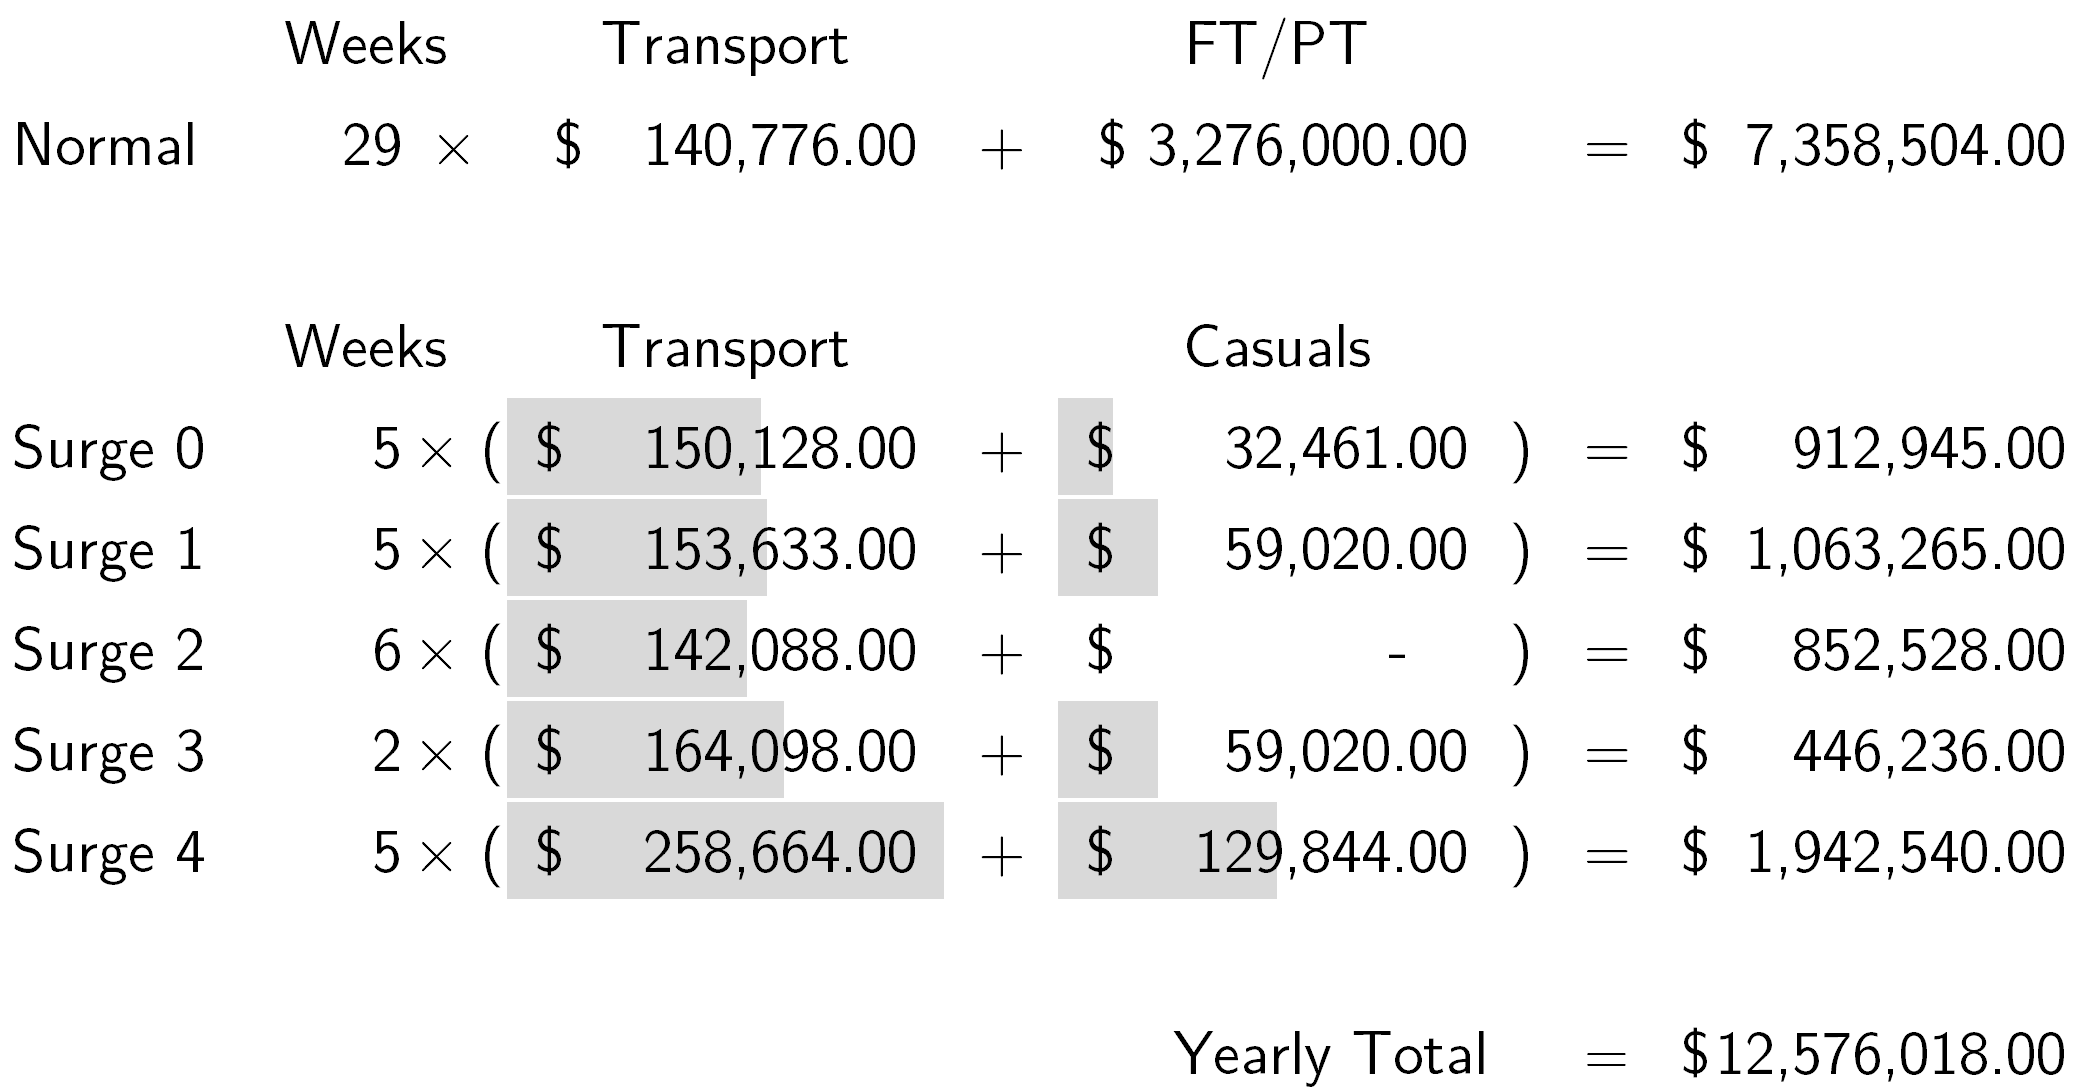
\includegraphics[width=33em]{table.PNG}

\section{General Observations}
While optimising the assignments with the data you provided us, we made 
the following observations.
\begin{itemize}
    \item The optimal solution to communication 9 uses no part-time teams, despite 
    them being used in communication 8. This is because the additional 
    capacity from full-time staff will be used during surge
     scenarios, reducing the need for expensive casual workers. Each casual worker only 
     handles 1 truckload, but costs 65\% as much as a full-time team which handles 
     9 truckloads. Note how 
     surge 2 can be handled by the only full-time staff.
    \item With communication 9, we have a fairly complete picture of WonderMarket's
    logistics needs and costs. Some DC capacities are never fully utilised, 
    but the model accounts for this and only assigns enough staff to handle 
    the required demand. This means if demand increases, you can simply employ more 
    staff (as long as DC capacity is sufficient). However, we would recommend
    re-evaluating the model to optimise for the new situation.
    \item With the construction of DC3 and DC5, your total capacity has increased 
    notably. Even the most demanding surge scenario, surge 4 with 164 truckloads,
    has 55 truckloads of spare capacity across DC1, DC2 and DC5.
    \item With that in mind, DC3 is nearing its capacity. There are at most  
    4 unused truckloads per week. In surge scenario 4, all of its 
    capacity is used. 
\end{itemize}

\section{Marginal Costs}
These are the effects of slight adjustments to the constraints 
you have provided us. These may be useful to improve your management of 
 distribution centres or logistics. 
\begin{itemize}
    \item With the notes on DC capacity above, increasing the DC1, DC2, DC3 or DC5's
    capacity by 1 does not affect the cost as the DC capacity is no longer a 
    limiting factor.
    \item If you can close one more DC to open a new site, you should close 
    DC1 and open DC6. This would reduce your yearly cost by \$853344 (\$16410.46 per week),
    to \$11722674 (\$225436.04 per week).
    \item The solution assigns 5 of the 10 stores to DC3. If DC3 could not be built, 
    your cost would be increased by \$1225564 yearly (\$23568.54 weekly) 
    to \$13801582 yearly (\$265415.04 weekly). Using DC0, DC1, DC2 and DC6 would 
    then be optimal.
\end{itemize}

\end{document}